%%
% The BIThesis Template for Bachelor Graduation Thesis
%
% 北京理工大学毕业设计(论文)第一章节 —— 使用 XeLaTeX 编译
%
% Copyright 2020 Spencer Woo
%
% This work may be distributed and/or modified under the
% conditions of the LaTeX Project Public License, either version 1.3
% of this license or (at your option) any later version.
% The latest version of this license is in
%   http://www.latex-project.org/lppl.txt
% and version 1.3 or later is part of all distributions of LaTeX
% version 2005/12/01 or later.
%
% This work has the LPPL maintenance status `maintained'.
%
% The Current Maintainer of this work is Spencer Woo.
%
% 第一章节

\chapter{前言}

\section{光线追踪简介}
光线追踪技术在影视特效中的运用已经十分广泛了。几乎所有的动画电影都是建立在光线追踪的算法之上的。近两年因为游戏硬件的发展,游戏行业也开始使用光线追踪技术来提高画面质量。

为了生成一个虚拟的画面,需要有两个要素,虚拟的场景和一个虚拟的镜头用来捕捉场景的光线,从而得到虚拟的画面。光线追踪就是光线从镜头出发,反向运动与场景中的物体发生碰撞,根据物体的特性不同经过折射、反射(漫反射、镜面反射)等运动方式,将物体的颜色进行叠加得到这束光线的最终颜色。

\section{黑洞简介}
在纯粹天体物理的研究方面,相对论宇宙的光线追踪方程几十年前就已经完善了。但是缺乏针对人视觉的高质量的渲染图,导致黑洞的视觉效果还停留在科学家的草稿里,很多人对黑洞并不了解.
\begin{enumerate}
    \item 黑洞 \\ 黑洞是一片引力强大到连光都无法逃脱的区域\cite{what_is_black_hole}。银河系的中心就是一个质量为太阳430万倍的黑洞\cite{galactic_center_bh},几乎所有的星系中心都是一个超大质量的黑洞;
    \item 奇点 \\ 黑洞的中心是一个密度无穷大的奇点,奇点的时空也无限扭曲。黑洞奇点是造成时空扭曲并形成黑洞视界的根源;
    \item 事件视界 \\ 黑洞的视界是使黑洞称为黑洞的区域,视界以内的信息都无法向外传递,因为没有向外的路径存在。本文研究的限制在视界以外的区域(exterior);
    \item 引力透镜 \\ 黑洞(事件视界)根据无毛定理,任何信息都不能从视界上发射出来,导致黑洞本身是不能被看到的。但黑洞会扭曲周围的时空,通过观察周围物质的运动可以“看”到黑洞。黑洞就像一个圆形或者近似圆形透镜,会使远处传来的平行光产生偏折。
\end{enumerate}

\section{黑洞可视化的现状}
一向追求真实的电影特效刚刚开始接受非平直时空的渲染。2009年的电影《星际迷航》中描绘的虫洞是一个扁平的圆环,而黑洞没有任何效果,直接消失得无影无踪。2014年的电影《星际穿越》第一次将球形的黑洞(视界)搬上荧幕,从那时候起科幻电影也开始重视真实的描述黑洞的物理特征。2017年的科幻剧《星际迷航:发现号》也开始使用球状的黑洞。当很多人通过影视作品了解到黑洞真正的样子后,就不能再用老旧刻板的印象来刻画黑洞了。

已经存在一些生成黑洞影像的开源渲染器,但这些渲染器存在一些诸如精度不高难以体现多重爱因斯坦环,或者使用近似的公式与实际的光线轨迹有较大差别等问题。

本文主要侧重于较高的渲染精度,来体现比较重要的几个黑洞特征。

NASA在过去十年偶尔会发布一些黑洞的渲染图\cite{nasa_2019_blackhole_visualization}\cite{raytraceusingstarcatalogue},但都没有渲染器的源代码公布。这个starless程序\cite{starless}是一个不错的渲染器。

\begin{figure}[htbp]
    \centering
    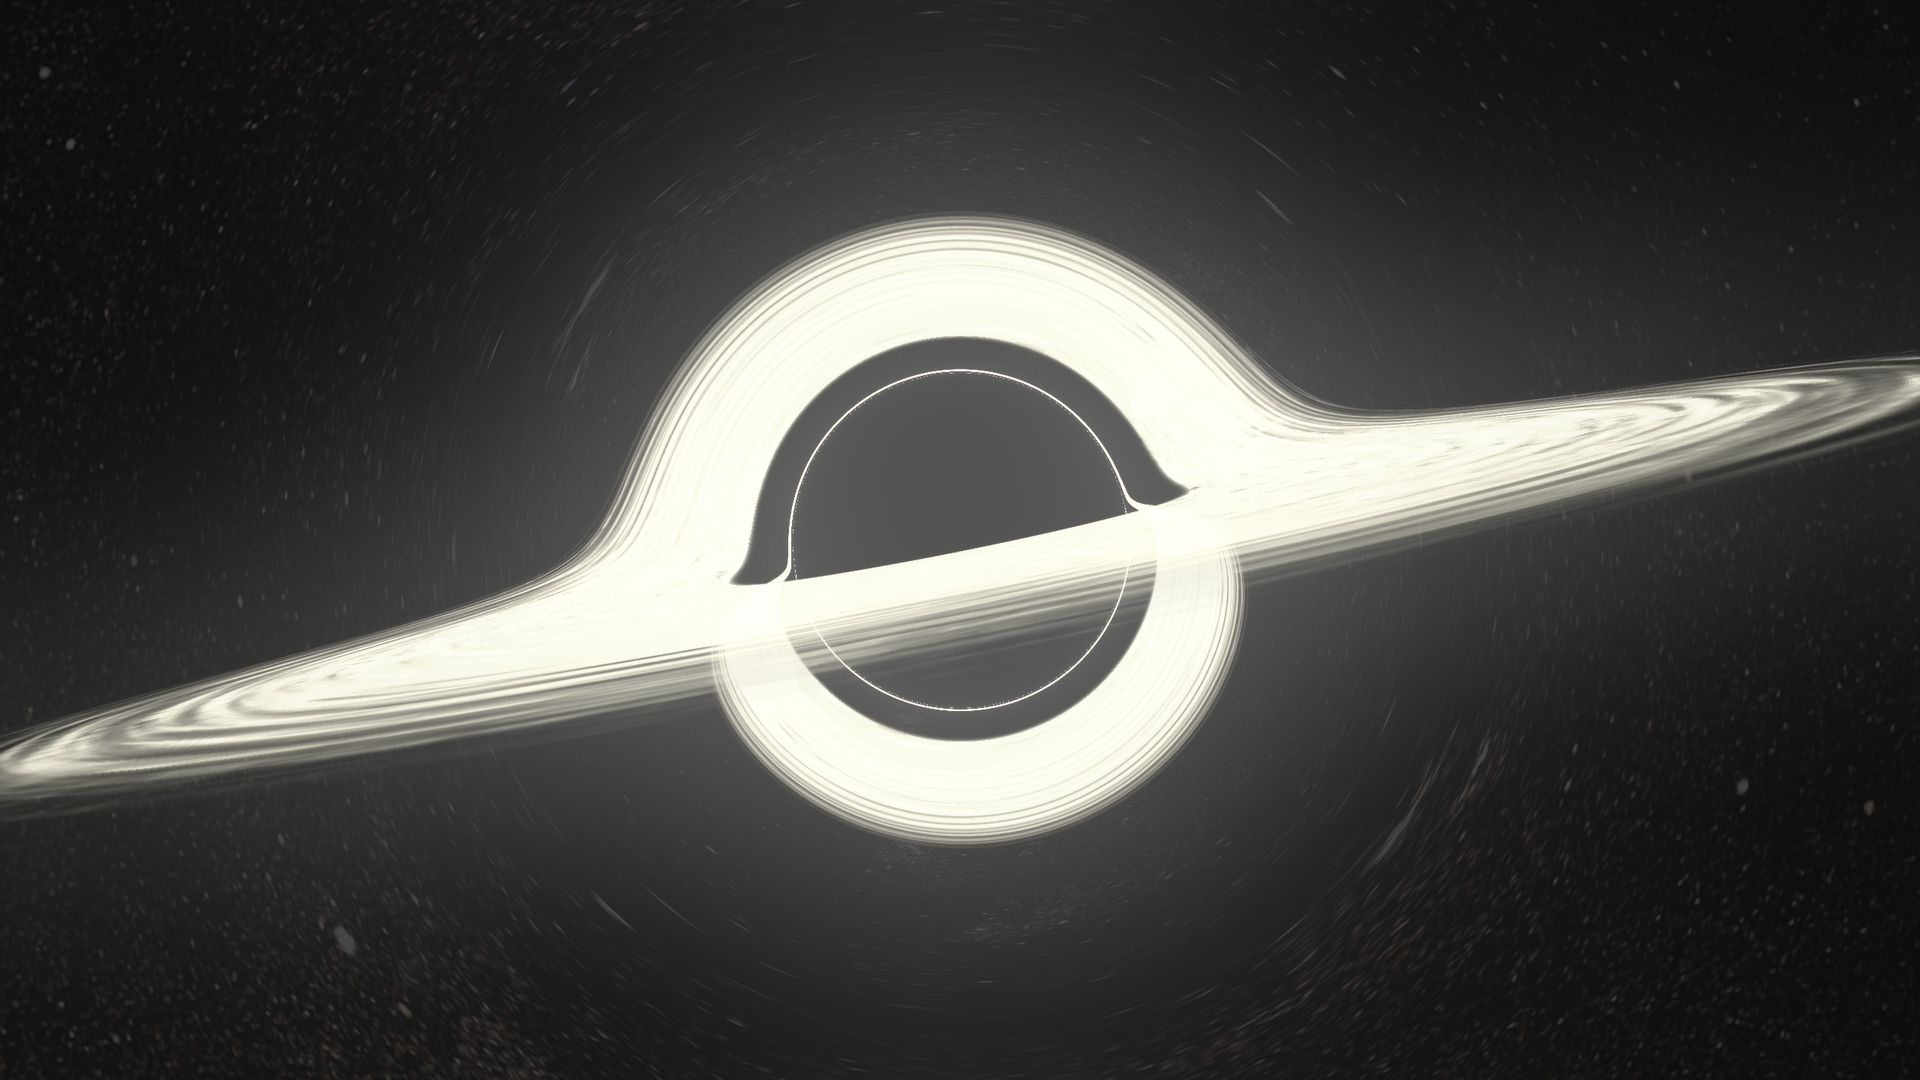
\includegraphics[scale=0.2]{images/starless_hd.jpg}
    \caption{starless生成的渲染图}\label{fig:starless_hd} % label 用来在文中索引
\end{figure}
通过对starless程序的研究认为它存在以下三个问题:
\begin{enumerate}
    \item 此渲染器的精度不够,没有办法看到贴近黑洞视界的光圈的景象;
    \item 此渲染器速度慢,上图分辨率是1080p,渲染时间需要4分钟左右,分辨率翻倍会让渲染时间指数上升;
    \item 此渲染器是用Python写的,因为Python第三方库分发不易的特点,程序易用性不足。
\end{enumerate}


\section{本论文的主要研究内容}
\subsection{论文结构}
第一章简述了本文的目的,介绍了黑洞与光线追踪技术。

第二章主要进行在广义相对论的理论下对光线的运动轨迹进行推导,得出一个易于计算而且适合场景渲染的公式。并对光线追踪过程中一些必要的步骤进行梳理,在二维平面上做一个简单的光线追踪模拟。第二章提到的算法是第三章的基础。

第三章利用第二章得出的公式与算法,实现一个设定场景下的光线追踪程序,实现黑洞可视化的目的。并尝试用不同的方法达到最快的渲染速度。
\subsection{创新点}
本设计主要尝试解决上述已有程序的问题:
\begin{enumerate}
    \item 程序可以拥有非常高的分辨率,在高分辨率的情况下还能保证细节;
    \item 程序的性能很高,渲染一个类似上述的1080p分辨率,有一个吸积盘的场景,在本人的笔记本电脑上渲染只需要20秒;
    \item 程序有用一个图形界面,可以比较容易的生成图片或者视频;
    \item 程序是跨平台的,可以在Windows、Linux下运行。
\end{enumerate}


